\documentclass[10pt]{article}
\usepackage{../../local}
\urlstyle{same}

\newcommand{\classcode}{Physics H195A}
\newcommand{\classname}{Physics Honors Thesis Proposal}
\renewcommand{\maketitle}{%
\hrule height4pt
\large{Yutong (Eric) Du \hfill \classcode}
\newline
\large{Proposal} \Large{\hfill \classname \hfill} \large{\today}
\hrule height4pt \vskip .7em
\small{Header styling inspired by CS 70: \url{https://www.eecs70.org/}}
\normalsize
}
\linespread{1.2}
\begin{document}
	%\maketitle
	\section{Background}

	Particle dark matter detection has been an ongoing field of research for 
	decades, and over time there have been many different proposed designs to build 
	a machine capable of detecting the weak interactions between hypothesized dark 
	matter particles and ordinary matter. As a non-collider detector, 
	experiments like SuperCDMS and TESSERACT use cryogenic solids and liquids 
	as target materials to detect the interactions between dark and ordinary 
	matter. 

	Currently, the detector operates by detecting collisions between cosmic particles 
	and the target atoms in the detector. When such a collision happens, a 
	small vibration, i.e., phonons, are generated, which propagate throughout the 
	material. Then, superconducting devices called Transition Edge Sensors (TES) detect 
	these vibrations, which are converted to electrical signals and read out. 

	This project I am interested in focuses on a new kind of phonon sensor, called a 
	kinetic inductance detector (KID).
	Similar to the TES, these are superconducitng circuits 
	placed onto the target material. 
	The motivation for coming up with a new detector is manyfold, but one simple reason 
	is that the physical circuitry for a KID-based detector is much simpler, making 
	it much easier to diagnose and fix issues when things malfunction. To add, 
	the components used largely consist of commercial RF hardware, which is much cheaper 
	than those used for TES. As a result, a system with KID-based detectors is 
	competitive for this and multiple other reasons, see \href{https://thesis.library.caltech.edu/15199/1/Chang_YenYung_2021.pdf}{here} for more details. 

	\section{KID-based detector}
	At its core, the KID is really nothing more than a simple LC circuit:
	\begin{center}
		\begin{circuitikz}[scale=1.5]
			\draw(0, 0) to (3, 0);
			\draw (1.5, 0) to[capacitor] (1.5, -0.5);
			\draw (1.5, -0.5) to (1, -0.5) to [vL] (1, -2); 
			\draw (1.5, -0.5) to (2, -0.5) to [capacitor] (2, -2);
			\draw (1, -2) to (2, -2);
			\draw (1.5, -2) to (1.5, -2.5);
			\draw (0, -2.5) to (3, -2.5);
		\end{circuitikz}
		\quad 
		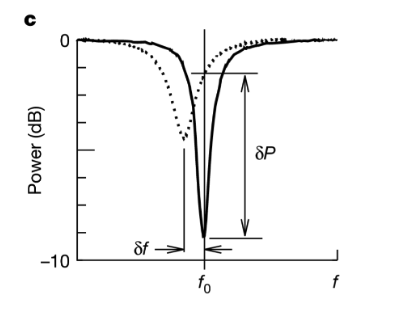
\includegraphics[scale=0.4]{freq_response.png}
	\end{center}
	Its frequency response is shown on the right, where we see a very narrow 
	dip at \( f = f_0 \), a parameter we can control. The dip at \( f = f_0 \) means 
	that this particular KID suppresses sine waves with exactly \( f = f_0 \), but 
	leaves other frequencies untouched. So, the idea for a KID-based 
	detector is as follows: we line many KIDs in series connected with a 
	feed line, each one calibrated to attenuate at a specific frequency 
	\( f = f_0 \). Then, we send a linear combination
	of sine waves at the frequencies we chose through the circuit, and read its 
	output. Under normal circumstances, this will return a suppressed signal. 
	Then, when a phonon is absorbed by the superconductor, it alters the value of 
	\( L \) slightly, causing a momentary shift in the frequency response. As a result, 
	the signal that used to be attenuated by that particular KID is now less 
	suppressed, producing a pulse in the signal we can detect. Depending on 
	the frequency of the detected signal, we can also determine which KID 
	was hit, and thereby reconstruct where the collision took place in the target 
	material. 
	
	\section{Project Description} 
	What was described above is an extremely idealized picture of what a KID-based 
	detector looks like. Unfortunately, current prototypes for this detector 
	has proven to be ineffective, one of the issues being the amount of impedance 
	interference present in the circuit. To illustrate this point, we 
	take a schematic of the full circuit, shown below:

	\begin{center}
		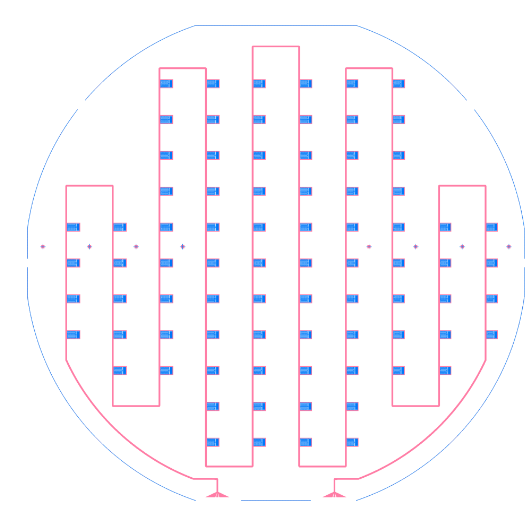
\includegraphics[scale=0.3]{feed_line.png}
		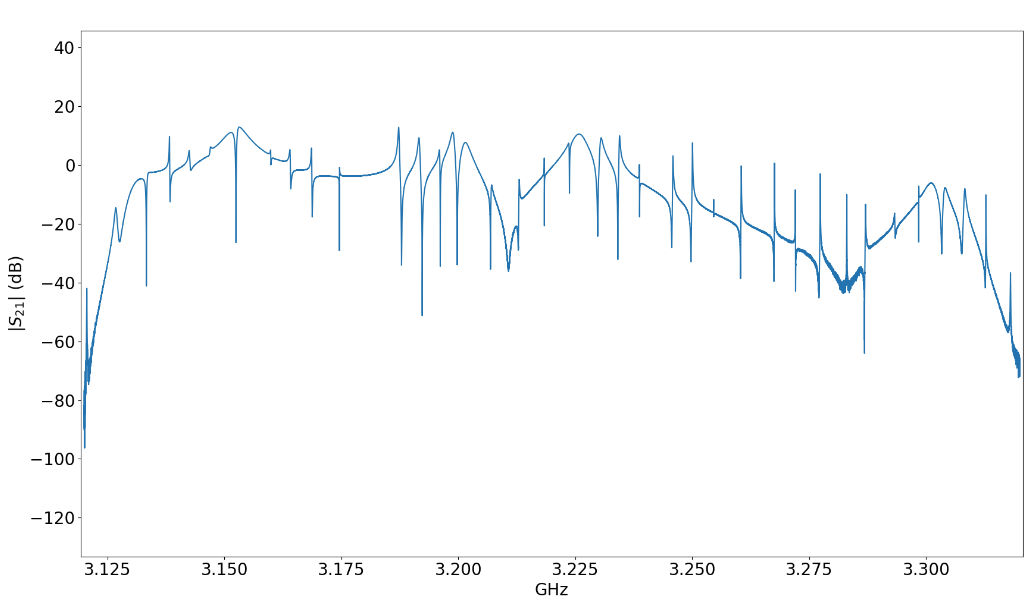
\includegraphics[scale=0.3]{exp.png}
	\end{center}
	The image on the left is the schematic, and its frequency response is shown on the right. 
	Each blue square represents a KID, and the red line represents the feed line
	that we send sine waves through. Currently, the issue with this implementation 
	is that whenever there is a sharp corner in the feed line, which causes interference 
	that distorts the frequency response of all KIDs. The evidence for this 
	distortion can be seen in the frequency response curve, as the degree 
	to which each KID attenuates the signal is non-uniform, and also the overall 
	shape of the curve (so disregarding the spikes from the KIDs) is not as uniform 
	as we would ideally want. As a result, these effects make some KIDs more 
	sensitive than others, and overall makes the device a weaker detector.  

	To solve this problem, we follow an approach developed by \href{https://ieeexplore.ieee.org/document/4752856}
	{Kim (2009)}. In the paper, they attempt to solve this issue by introducing
	a phenomenon called "slow wave compensation", shown below:

	\begin{center}
		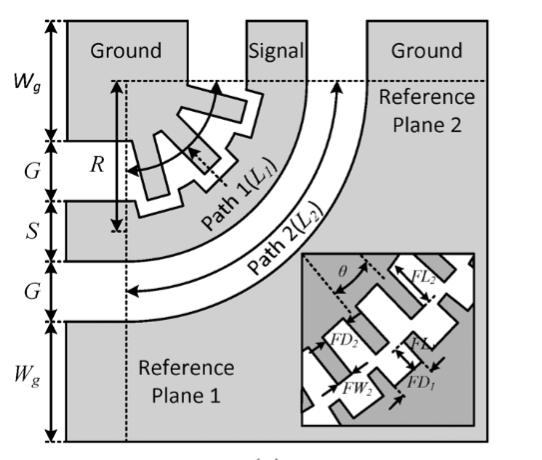
\includegraphics[scale=0.6]{slow_wave.png}
	\end{center}

	In essence, the interference in the system is thought to be caused by a phase 
	difference between the two travelling waves, since the wave along the inner 
	radius of the corner travels less distance than the outer. The introduction 
	of "forks" on the inner track generates some capacitance, and serves to 
	slow the inner wave down so that both waves remain in phase upon exit. The required 
	capacitance to do this is also well known, since we know exactly how much further 
	the outer wave travels. 
	This paper also provided some very basic simulations of the proposed solution, and 
	it has shown to greatly reduce the effects of impedance interference, which shows 
	that this method is indeed promising. 

	For this honors project, our goal is to further develop these simulations to 
	closely replicate the detector geometry, and ultimately try to understand the 
	interactions that happen between the feed line and its surroundings. Investigation 
	into this not only helps us get one step closer to developing new ways to detect
	dark matter, but it also has large implications on other fields as well, since 
	cryogenic RF transmission lines are employed in other cryogenic devices such as quantum 
	computers. 
	My project will be largely done in an FEA software called Ansys HFSS, a program 
	specially designed to simulate 3D electromagnetic systems. I will be primarily 
	working with Dr. Yen-Yung Chang, co-sponsored by Prof. Matt Pyle. 
	

\end{document}
